\section{Experimental Results}
\label{experiment}

\subsection{Dataset}
\label{experiment:dataset}
We experiment on four trajectory datasets provided by \cite{ijcai15} that were
extracted from Yahoo! Flickr Creative Commons 100M (a.k.a. YFCC100M) dataset~\cite{thomee2016yfcc100m} 
using metadata of photos and videos such as geographical locations, timestamps, user identifications etc.
Statistics of the four trajectory datasets are described in table \ref{table:data}.
%
The time that a user arrived a POI was approximated by the time the first photo taken by the user at that POI,
similarly, the time that a user leaved a POI was approximated by the time the last photo taken by the user at 
that POI \cite{ht10, ijcai15}.
An example of trajectory with four POIs from Toronto dataset was shown in figure \ref{fig:traj}, 
%TODO: explain what is a POI/photo in the figure
where the four colored marker icons represent the four POIs, 
and the colored round icons represent a sample of photos assign to these POIs.


\begin{figure}
\centering
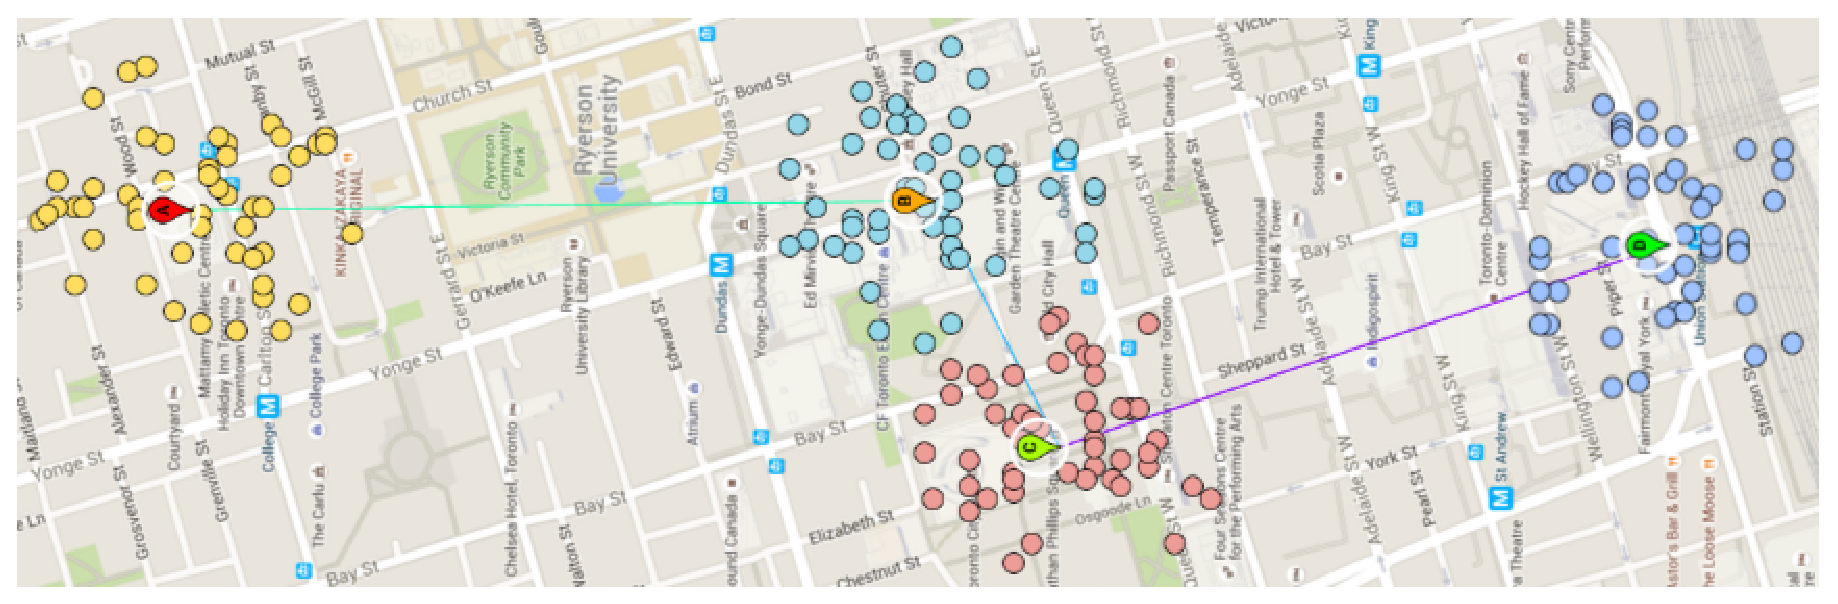
\epsfig{file=traj_eg.eps, width=3.5in}
\caption{An example of trajectory with four POIs}
\label{fig:traj}
\end{figure}

\begin{table*}
\centering
\begin{tabular}{lrrrrr} \hline
\textbf{Dataset} & \textbf{\#Photos} & \textbf{\#POI Visits} & \textbf{\#Trajectories} & \textbf{\#Users} \\ \hline
Edinburgh & 82,060 & 33,944 & 5,028 & 1,454 \\ 
Glasgow & 29,019 & 11,434 & 2,227 & 601 \\ 
Melbourne & 94,142 & 23,995 & 5,106 & 1,000 \\ 
Osaka & 392,420 & 7,747 & 1,115 & 450 \\ 
Toronto & 157,505 & 39,419 & 6,057 & 1,395 \\ 
\hline
\end{tabular}
\caption{Statistics of trajectory dataset}
\label{table:data}
\end{table*}


\subsection{Evaluation}
We use leave-one-out cross validation to evaluate different trajectory recommendation algorithms,
i.e., when evaluating a trajectory of a specific user, all other trajectories of this user as well as 
all trajectories of other users were used to train the recommendation algorithms.

In addition, we compared the experimental results on four trajectory datasets among 
the following recommendation algorithms.
\begin{itemize}
\item \textsc{Random}: choose POIs uniformly at random (without replacement) 
      from the set of POIs $\mathcal{P} \setminus \{p_s, p_e \}$ to visit.
\item \textsc{PersTour}\cite{ijcai15}: personalised trajectory recommendation algorithm with time budget constraint,
      the trade-off parameter was $0.5$.
\item \textsc{PersTour-L}: the same setting as \textsc{PersTour} but with time budget constraint replaced with the 
      total number POIs to visit, i.e., $L$.
\item \textsc{PoiPopularity}: choose POIs according to the ranking based on POI popularity only.
\item \textsc{PoiRank}: choose POIs according to the ranking based on POI features described in section \ref{method:ranking}.
\item \textsc{Markov}: recommend trajectory according to the factorized transition matrix described in section \ref{method:transition},
      using Viterbi algorithm to compute the most likely trajectory with respect to constraint $(p_s, p_e, L)$.
\item \textsc{MarkovPath}: the same as \textsc{Markov}, but with extra restriction that 
      no sub-tours exist in the recommended trajectory.
\item \textsc{Rank+Markov}: combining POI ranking and the factorized transition matrix and use algorithm \ref{algo:dp} to 
      compute the most likely trajectory with respect to constraint $(p_s, p_e, L)$.
\item \textsc{Rank+MarkovPath}: the same as \textsc{Rank+Markov}, but with extra restriction that 
      no sub-tours exist in the recommended trajectory.
\item \textsc{StructuredSVM}: structured prediction algorithm using POI rankings as well as transition probabilities
      between POIs to recommend trajectory as described in section \ref{method:structured}.
\end{itemize}

% Parameters
For all algorithms that utilizing ranking probabilities of POIs, namely, \textsc{PoiRank}, \textsc{Rank+Markov} and 
\textsc{Rank+MarkovPath}, the regularization parameter of rankSVM was $10$.
The discretization parameters used to factorize the transition probabilities between POIs was $5$, namely,
discretizing POI features into $5$ bins and clustering POIs to $5$ clusters according to the geographical coordinates.
The trade-off parameters $\alpha$ was set to $0.5$ in both \textsc{Rank+Markov} and \textsc{Rank+MarkovPath} algorithms.
The regularization parameter to train \textsc{StructuredSVM} was $1$.


\subsection{Results}
% tell the story: justify each row in the table, make comparison.
The F$_1$-scores of the nine algorithms on all four datasets are shown in table \ref{table:f1}.
The information utilized by these algorithms except \textsc{Random} range from POI information and query information 
of trajectories to transition patterns between different POIs and so on, table \ref{table:character} summarize the 
characteristics of all the nine algorithms.

From table \ref{table:f1}, one can observe that all algorithms that capture POI specific information significantly 
outperform the one that does not use it, namely the \textsc{Random} baseline algorithm, 
which indicates the POI specific information is very helpful for recommending trajectories.
%
% time constraint is better than length constraint
Another observation is \textsc{PersTour} get much better trajectory F$_1$-scores on all four datasets 
than \textsc{PersTour-L}, which is equivalent to \textsc{PersTour} except the total number of POIs was used to 
constrain recommendation, which means, at least for \textsc{PersTour}, the total time consumed in a trajectory
provides more helpful information than purely the number of POIs one should visit, and indicates that recommendation
algorithms which use the number of POIs instead of the time consumed might not perform as well.
%
% comparison between ijcai and other methods
However, algorithms that did not utilize the total time consumed in a trajectory can outperform the one that 
used this information (i.e., \textsc{PersTour}) on three out of four datasets, 
by learning to rank POIs based on informative POIs features and exploiting the transition patterns between POIs.

% strong performance of POI popularity based ranking on Edinburgh data
POI features seems to be very helpful for recommending trajectories.
In particular, recommendation based on ranking POI popularity only 
(i.e., \textsc{PoiPopularity}) yields very good performance on two out of four datasets, 
especially on Edinburgh dataset, where it surprisingly outperforms all 
other algorithms, including those much more sophisticated than this simple ranking method.
%
% strong performance of POI feature based ranking on Toronto and Glasgow data
Furthermore, \textsc{PoiRank} performs very well in three out of four datasets, 
especially on Toronto dataset, where it got better results than any other methods, 
while on both Edinburgh and Glasgow datasets, it was the second best performer, 
which indicates that learning to rank is very helpful when recommending trajectories.

% the performance of transition-only methods
Recommendation by exploiting only transition patterns did not performs quite well,
but when supported by learning to rank, it improves a lot, which results the best performer on Osaka dataset and
the third best performer on all other datasets, namely \textsc{Rank+MarkovPath}.

% sub-tours hurt
In addition, we found that sub-tours hurt trajectory recommendation when compare the performance between
\textsc{Markove} and \textsc{MarkovPath} as well as between \textsc{Rank+Markov} and 
\textsc{Rank+MarkovPath}, while the latter algorithms got an additional restrict that no sub-tours 
occur in recommended trajectories.
% 
% why structured prediction didn't work very well
This discovery could also be the reason that the sophisticated structured prediction algorithm, 
i.e., \textsc{StructuredSVM}, can not perform better than the best performer among the various algorithms
that exploiting POI rankings and/or transition patterns.


% performance comparison in terms of tau
On the other hand, when compare the performance of different recommendation algorithms in terms of trajectory $\tau$
which measures the quality of visiting orders of POIs in recommended trajectories,
as shown in table \ref{table:tau}
\footnote{We can not compute trajectory $\tau$ for \textsc{PersTour} because the number of POIs in recommend trajectory 
is not guaranteed to equal the number of POIs in real trajectory.},
\textsc{StructuredSVM} became the best performer in three out of four datasets,
this is expected as \textsc{StructuredSVM} can tune much more parameters than other algorithms when training,
which means it can utilize the transition patterns between POIs better,
as a result, when POIs in a recommended trajectory also appear in the ground truth, 
there is a better chance that the visiting order among these POIs are also consistent with 
that in the real trajectory.

% 
The last interesting observation that we want point out is the performance of \textsc{PoiPopularity} algorithm
on Edinburgh dataset, where it yields the best performance in terms of trajectory F$_1$-score and 
also get very good performance, almost comparable to the best performer in terms of trajectory $\tau$.
This observation indicates that most tourists visiting Edinburgh not only just visiting
places that are very popular, but also follow similar visiting orders when visiting these places.

\begin{table*}
\centering
\begin{tabular}{l|ccccc} \hline
 & Edinburgh & Glasgow & Melbourne & Osaka & Toronto \\ \hline
\textsc{Random} & $0.570\pm0.139$ & $0.632\pm0.124$ & $0.558\pm0.149$ & $0.621\pm0.117$ & $0.621\pm0.128$ \\
\textsc{PersTour}\cite{ijcai15} & $0.656\pm0.223$ & $\mathbf{0.802\pm0.213}$ & $0.491\pm0.211$ & $0.702\pm0.230$ & $0.720\pm0.215$ \\
\textsc{PersTour-L} & $0.651\pm0.143$ & $0.660\pm0.102$ & $0.578\pm0.140$ & $0.691\pm0.138$ & $0.642\pm0.112$ \\
\textsc{PoiPopularity} & $\mathbf{0.701\pm0.160}$ & $0.745\pm0.166$ & $0.621\pm0.136$ & $0.661\pm0.128$ & $0.679\pm0.120$ \\
\textsc{PoiRank} & $\mathit{0.694\pm0.157}$ & $\mathit{0.777\pm0.171}$ & $\mathbf{0.626\pm0.137}$ & $0.679\pm0.112$ & $\mathbf{0.748\pm0.166}$ \\
\textsc{Markov} & $0.629\pm0.172$ & $0.714\pm0.168$ & $0.577\pm0.168$ & $0.679\pm0.162$ & $0.663\pm0.157$ \\
\textsc{MarkovPath} & $0.678\pm0.148$ & $0.731\pm0.167$ & $0.596\pm0.147$ & $0.706\pm0.154$ & $0.689\pm0.140$ \\
\textsc{Rank+Markov} & $0.642\pm0.171$ & $0.736\pm0.176$ & $0.598\pm0.169$ & $0.701\pm0.171$ & $0.689\pm0.170$ \\
\textsc{Rank+MarkovPath} & $0.684\pm0.151$ & $0.760\pm0.170$ & $\mathit{0.625\pm0.150}$ & $\mathbf{0.719\pm0.161}$ & $0.724\pm0.152$ \\
\textsc{StructuredSVM} & $0.659\pm0.186$ & $0.727\pm0.173$ & $0.597\pm0.171$ & $\mathit{0.715\pm0.170}$ & $\mathit{0.728\pm0.186}$ \\
\hline
\end{tabular}
\caption{Performance comparison on four datasets in terms of trajectory F$_1$-score. 
         For each dataset (i.e., a column), the best method is shown in bold, the second best is shown in italic.}
\label{table:f1}
\end{table*}


\begin{table*}
\centering
\begin{tabular}{l|ccccc} \hline
 & Edinburgh & Glasgow & Melbourne & Osaka & Toronto \\ \hline
\textsc{Random} & $0.259\pm0.155$ & $0.318\pm0.165$ & $0.248\pm0.148$ & $0.305\pm0.145$ & $0.309\pm0.166$ \\
\textsc{PersTour-L} & $0.350\pm0.206$ & $0.349\pm0.163$ & $0.267\pm0.144$ & $0.415\pm0.243$ & $0.329\pm0.158$ \\
\textsc{PoiPopularity} & $\mathit{0.421\pm0.257}$ & $0.503\pm0.296$ & $0.310\pm0.179$ & $0.361\pm0.194$ & $0.378\pm0.203$ \\
\textsc{PoiRank} & $0.410\pm0.246$ & $\mathbf{0.557\pm0.311}$ & $0.315\pm0.187$ & $0.367\pm0.162$ & $\mathit{0.501\pm0.294}$ \\
\textsc{Markov} & $0.404\pm0.229$ & $0.472\pm0.282$ & $0.296\pm0.191$ & $0.442\pm0.259$ & $0.406\pm0.231$ \\
\textsc{MarkovPath} & $0.390\pm0.235$ & $0.479\pm0.292$ & $0.293\pm0.187$ & $0.445\pm0.268$ & $0.401\pm0.235$ \\
\textsc{Rank+Markov} & $0.411\pm0.237$ & $0.522\pm0.293$ & $\mathbf{0.344\pm0.202}$ & $\mathit{0.475\pm0.278}$ & $0.449\pm0.263$ \\
\textsc{Rank+MarkovPath} & $0.395\pm0.238$ & $\mathit{0.523\pm0.303}$ & $0.327\pm0.214$ & $0.470\pm0.284$ & $0.455\pm0.268$ \\
\textsc{StructuredSVM} & $\mathbf{0.423\pm0.264}$ & $0.505\pm0.282$ & $\mathit{0.335\pm0.215}$ & $\mathbf{0.499\pm0.293}$ & $\mathbf{0.511\pm0.312}$ \\
\hline
\end{tabular}
\caption{Performance comparison on four datasets in terms of $\tau$.
         For each dataset (i.e., a column), the best method is shown in bold, the second best is shown in italic.}
\label{table:tau}
\end{table*}


\begin{table*}
\centering
\begin{tabular}{l|cccccc} \hline
                                    & Query    & POI      & Transition & No sub-tours & Joint    \\ \hline
\textsc{Random}                     & $\times$ & $\times$ & $\times$   & $\times$     & $\times$ \\ 
\textsc{PersTour}\cite{ijcai15}     & $\times$ & $\surd$  & $\times$   & $\surd$      & $\times$ \\
\textsc{PersTour-L}                 & $\times$ & $\surd$  & $\times$   & $\surd$      & $\times$ \\
\textsc{PoiPopularity}              & $\times$ & $\surd$  & $\times$   & $\times$     & $\times$ \\ 
\textsc{PoiRank}                    & $\surd$  & $\surd$  & $\times$   & $\times$     & $\times$ \\
\textsc{Markov}                     & $\times$ & $\surd$  & $\surd$    & $\times$     & $\times$ \\
\textsc{MarkovPath}                 & $\times$ & $\surd$  & $\surd$    & $\surd$      & $\times$ \\
\textsc{Rank} + \textsc{Markov}     & $\surd$  & $\surd$  & $\surd$    & $\times$     & $\times$ \\
\textsc{Rank} + \textsc{MarkovPath} & $\surd$  & $\surd$  & $\surd$    & $\surd$      & $\times$ \\
\textsc{StructuredSVM}              & $\surd$  & $\surd$  & $\surd$    & $\times$     & $\surd$  \\ \hline
\end{tabular}
\caption{Characteristics of different algorithms}
\label{table:character}
\end{table*}



\subsection{Avoid Peeking}
When working with machine learning algorithms, to make sure the reported performance is a good approximation
of the generalization performance, it is critical to prevent information in test set from leaking into
training set.
Many algorithms in the above comparison utilizing both learning to rank and factorized transition matrix,
e.g., \textsc{Rank+Markov}, \textsc{Rank+MarkovPath} and \textsc{StructuredSVM},
both of them need to be trained or parameters be estimated before being utilized in other algorithms.
Features such as popularity of a POI, the number of visits of a POI and the average visit duration at a POI are
determined by not only the POI itself but also trajectories in training set, let's call them aggregated features as they are 
computed by aggregating a set of trajectories.
To make sure the prediction performance is reliable, it is very important to exclude trajectories in test set 
when computing aggregated features.
Unfortunately, it is quite easy, especially when utilizing multiple levels of machine learning models,
to use all data, including those in test set, to compute aggregated features and many researchers and 
practitioners did not realize some bits of information in test set were leaked into training set via these aggregated features.

%One may argue that many of these features will not change much when computed with or without data in test set,
%but in certain areas, such as aerodynamics, some decisions are very sensitive to the quantity of certain features.
%Nevertheless, the exact impact still needs further investigation.


